%
% Introduction
\chapter{Introduction} \label{chap::intro}%
There exist many situations in the world which are not safe, where a human is sent to help. Exploring the terrains of nuclear disasters, searching in a house on fire and clearing mine fields are all examples of this. Technology has extended the human's hand through history to a point where nowadays some people are wondering if we have almost hit the limits of fishing Mother Nature's pond of technology.  Safety standards in both professional and personal environments have greatly improved with the help of knowledge and technology. As is noticeable from the videos of Boston Dynamics going viral all over the world, legged robots, and more specifically humanoid robots, become more in a developed stage. However, comparing with the human physical capabilities, humanoid robots are still at most in a child phase.  The usefulness of these devices and the growth opportunities are a clear motivation to improve them.
\section{Motivation}
The walking humanoid robot system is highly complex. It deals with nonlinear multibody dynamics, complex kinematics, hybrid dynamics between switching ground contacts, unilateral friction-limited contact constraints and actuation limitations. Past research has approached nonlinearities with a linearized description of a walking robot \cite{kajita1992dynamic, pratt2006capture, koolen2012capturability} and has tackled joint level complexities by separating high level and joint level control \cite{kuindersma2016optimization, koolen2016design}. The planning problem of a walking gait has often been tackled by separating the footstep plan from the body motion plan \cite{chestnutt2005footstep,deits2014footstep,englsberger2014trajectory}. Although all these methods break the complexity of the system down and give a better approximation of how it will behave dynamically, often still a lot of assumptions are made. Linearization of the model has the advantage of giving a relatively simple measure, that can have a closed form solution in planning problems and that can be used in linear control. In Figure \ref{fig:3dlipfootinertiaz0} the basic model that is often considered is shown. The robot is modeled as a \ac{LIP} with constant height, were the foot and body inertia can be used for control. Recently research has been done in taking the constant height assumption away \cite{hopkins2014humanoid,liu2015trajectory, koolen2016balance, gao2017increase,nguyen2017dynamic, caron2018capturability}, but application of varying height models in control and planning is not yet proven to be successful. 
\section{Objective}
In this literature survey, the focus is to find how \ac{CoM} height variations are used in dynamic planning and control of a bipedal robot, with the goal of improving the dynamical behavior over rough, but also flat, terrain and improving robustness properties against disturbances. \\
Publications are compared based on several aspects. The needed underlying planning and control strategies for the presented methods play an important role, as they are related to the possibilities of application. The differences between \ac{2D} and \ac{3D} based methods can be pointed out and the differences between methods that require a predefined footstep plan and step timing in contrast to methods that define those. Computation times of the methods are compared, as they play an important role in real-time use. Presented results can be evaluated on the contribution to theory and application, where improvements or differences with respect to existing approaches are pointed out. In the case of control, robustness properties of the discussed strategy can be considered. As an example, strategies that fit a predefined footstep plan and that are presented in \ac{3D} are more likely to be applicable than a \ac{2D} strategy that defines the footsteps by the method itself, as most humanoids require a predefined footstep plan and rely on \ac{3D} dynamical models. \\
Even though the research area of focus is exploring the effects of varying height, a global study is done on humanoid robotics research in general, as it is important to understand which strategies are used in aspects that are related to the problem. \\
In Chapter \ref{chap:modeling}, a brief overview is given of basic humanoid walking related models and terminology. In Chapter \ref{chap:planningcontrol}, a general review is conducted on the current planning, control and state estimation strategies in humanoid robotics. Special attention is given to papers that were applied to Boston Dynamics' Atlas or NASA's Valkyrie at IHMC, as research is conducted and hopefully applied at this institute. In Chapter \ref{chap:varyingheight}, a full in-depth study is performed on publications that address \ac{CoM} height variation directly. In Chapter \ref{chap:conclusion}, a conclusion is made on the literature study and a goal for the research project is formulated. Information and ideas from different publications are tied together to attempt to formulate a balanced insight in the possibilities and concerns to tackle the problem.
\begin{figure}[h]
\centering
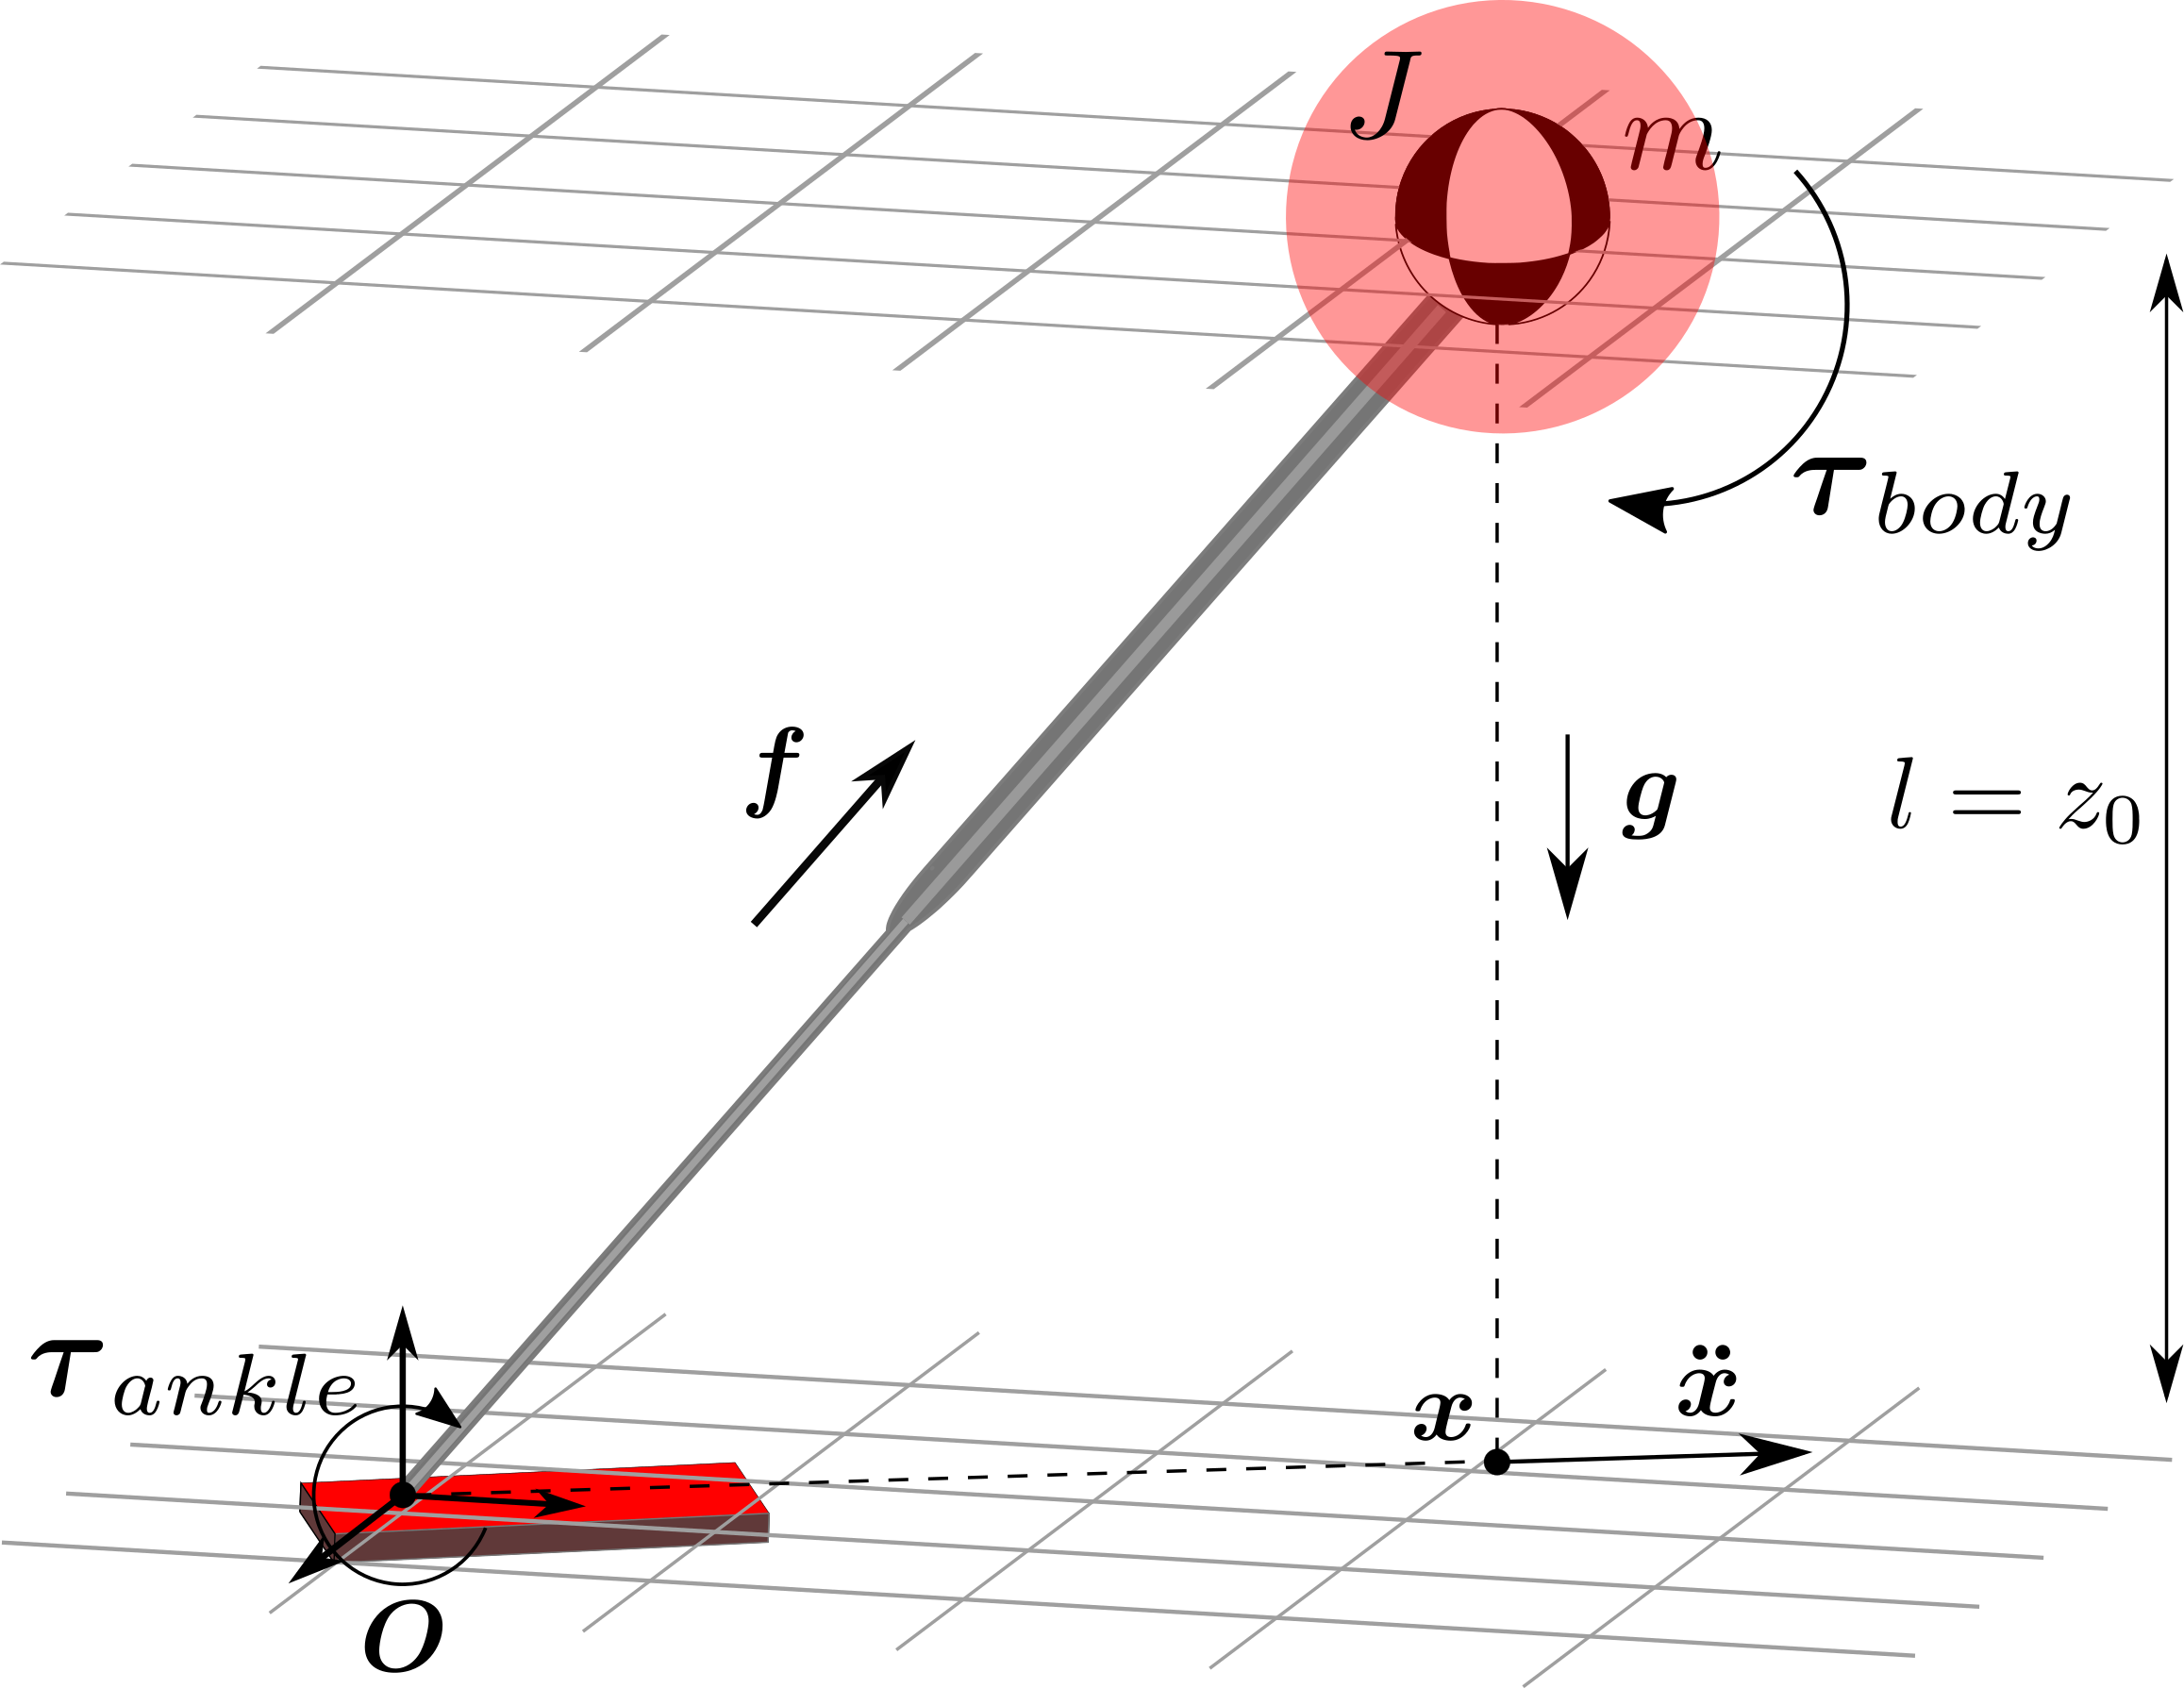
\includegraphics[width=0.5\textwidth]{STYLESTUFF/3DCoMfootinertiaz0.png}
\caption{\ac{3D} motion of \ac{LIP} model with foot at the base and a mass with inertia at the tip. The \ac{CoM} moves at constant height.}
\label{fig:3dlipfootinertiaz0}
\end{figure}




